\documentclass[a4paper,12pt]{report}
\usepackage{a4wide}

%\documentclass[a5paper,10pt]{book}
%\usepackage[top=23mm, bottom=18mm, left=15mm, right=25mm]{geometry}
%\geometry{papersize={170mm,220mm}}


\usepackage[utf8x]{inputenc}
\usepackage[danish]{babel}

\usepackage{xr-hyper} %Externe hyper-ref
\usepackage[colorlinks=true, hyperindex=true, linkcolor=minmblaa, citecolor=minmblaa, urlcolor=minmblaa]{hyperref}
\hypersetup{colorlinks=true,filecolor=minmblaa,bookmarksnumbered=true} %Til hyperreferencer. Referencer med farver
\usepackage{needspace} % giver mulighed for at kræve at der skal være et antal tomme linier på siden før ellers indsættes et sideskift.
\usepackage{framed} %Bokse
\usepackage{wrapfig}

\usepackage{amsmath,amsfonts,amssymb,amsthm,mathtools} %Matematikpakker

\setlength{\parindent}{0mm} %Ingen Indhak i første linje i afsnit

\usepackage{color} %Farvepakke

\usepackage{array}
\usepackage{colortbl}
\usepackage{multirow} %Til at flette rækker i tabeller.

\usepackage{verbatim,mhchem}



	% DOWNLOAD FRA: http://sarovar.org/frs/?group_id=52&release_id=97
	% Læg i directory for hoved TEX fil
%\usepackage[draft]{pdfdraftcopy}
%\draftstring{Licens: Kasper Langt Mellemnavn Skårhøj}
%\draftfontsize{30}
	%\draftfontfamily{hlh}
	%\draftangle{45}
	%\definecolor{mycolor}{rgb}{.825,.855,1}
	%\draftcolor{mycolor}
	%\draftfontattrib



% = Sidehoved =
\usepackage{fancyhdr}
\pagestyle{fancy}
\renewcommand{\sectionmark}[1]{\markright{\protect\titlegraphic{dturoed}\textcolor{dtugraa}{\thesection~\MakeUppercase{#1}}}} % \thesection.\
\fancyhead{}
\fancyfoot{}
\fancyhead[R]{\titlefont\thepage}
\fancyhead[C]{}
\fancyhead[L]{\titlefont \small eNote \MakeUppercase{~\thechapter}~\hspace*{1ex}\rightmark}
\renewcommand\headrulewidth{0pt}
\fancypagestyle{plain}{\fancyfoot[C]{}}% {\titlefont\footnotesize\thepage}}
\setlength{\headheight}{15pt}


% = Længder
%\newlength{\envtblsep}\setlength{\envtblsep}{1\FrameSep}
\newlength{\obsl}\setlength{\obsl}{\textwidth-1.2cm-13.2pt}

% Includes:

% =     Fonts (select one)    =
\usepackage{mathpazo}\linespread{1.05} % Palatino needs more leading (space between lines)
\usepackage{bm} % bold math, must be loaded after the fontpackages

% % Til overskrifter
\DeclareTextFontCommand{\th}{\fontencoding{T1}\fontfamily{phv}\fontseries{b}\selectfont}
\newcommand\titlefont{\fontencoding{T1}\fontfamily{phv}\selectfont}


% =     PGF grafik      =
\usepackage{tikz}
\newcommand\titlegraphic[1]{%
\tikz[baseline] %
\draw[thick,color=#1]
(0pt  ,-0.25em) -- (0pt  ,0.85em)
(2.5pt,-0.25em) -- (2.5pt,0.85em)
(5pt  ,-0.25em) -- (5pt  ,0.85em)
(7.5pt,-0.25em) -- (7.5pt,0.85em);\hspace*{0.8ex} %
}

\newcommand\titlegraphicwide[1]{%
\tikz[baseline] %
\draw[line width=0.8mm,color=#1]
(0pt  ,-0.25em) -- (0pt  ,0.85em)
(4.5pt,-0.25em) -- (4.5pt,0.85em)
(9pt  ,-0.25em) -- (9pt  ,0.85em)
(13.5pt,-0.25em) -- (13.5pt,0.85em);\hspace*{0.8ex} %
}


% =      Title Layout      =
\usepackage{titlesec}
\makeatletter
\titleformat{\chapter}
	[display] % Shape
	{\titlefont\Huge\flushleft} % Title and label format
	{\titlefont\LARGE\bfseries \titlegraphicwide{dturoed}\textcolor{dtugraa}{\@chapapp~\thechapter}} % label
	{0.9em} % label/title separation
	{} % before code
	[] % after code
\makeatother
\titleformat{\section}
	[hang] % Shape
	{\titlefont\Large\flushleft} % Title and label format
	{\thesection} % label
	{0.9em} % label/title separation
	{} % before code
	[] % after code
\titleformat{\subsection}
	[hang] % Shape
	{\titlefont\large} % Title and label format
	{\thesubsection} % label
	{0.9em} % label/title separation
	{} % before code
	[] % after code
\titlespacing{\subsection}{0pt}{*6}{*1.5}
\titleformat{\subsubsection}
	[hang] % Shape
	{\titlefont} % Title and label format
	{\thesubsubsection} % label
	{0.9em} % label/title separation
	{} % before code
	[] % after code



% = Farver
\definecolor{dturoed}{rgb}{0.6, 0.0, 0.0}
\definecolor{dtugraa}{rgb}{0.5, 0.5, 0.5}	% Lidt mørkere. Korrekt = 0.4
\definecolor{mingroenstreg}{rgb}{0.4,0.8,0}	% Sekundærfarve 14 : 102/204/0	(Forårsgrøn) -> Eksempler
\definecolor{mingroen}{rgb}{0.32,0.64,0}		% Sekundærfarve 14, 80% mørkere (tekst)
\definecolor{minorangestreg}{rgb}{1,0.6,0}		% Sekundærfarve 1 : 255/153/0	(Orange) -> Opgaver
\definecolor{minorange}{rgb}{0.8,0.48,0}		% Sekundærfarve 1 , 80% mørkere (tekst)

\definecolor{minblaa}{rgb}{0.2,0.4,0.8}	% Sekundærfarve 13 , 51/102/204 	( Blå -> Definitioner etc)
\definecolor{minmblaa}{rgb}{0.16,0.32,0.64}	% Sekundærfarve 13 , 80% mørkere (tekst)
\definecolor{thmbackground}{rgb}{0.97,.97, 0.99}	% Farve 13 - lys baggrund

\definecolor{mingraastreg}{rgb}{.5,.5,.5}
\definecolor{hvadbackground}{rgb}{0.97,.97, 0.97}
\definecolor{sumgul}{rgb}{1,1,.8}

\definecolor{hjmopgfarve}{rgb}{.96,1,.96}


% = Counter
\newcounter{evncount}[chapter]
\setcounter{evncount}{0}
\renewcommand{\theevncount}{\thechapter.\arabic{evncount}}
\renewcommand{\theequation}{\thechapter-\arabic{equation}}


% = Eksempler = example =
\newenvironment{example}[1][]{
	\refstepcounter{evncount}
	\setlength{\obsl}{\textwidth-1.2cm-13.2pt-9pt} % fix width of the info envirnment%
	\def\FrameCommand{ 
		\textcolor{mingroenstreg}{\vrule width 4pt} 
		\hspace{5pt} 
	}%
	\MakeFramed{\advance\hsize-\width \FrameRestore}%
	\needspace{3\baselineskip}
	\titlegraphic{mingroen}
	\textcolor{mingroen}{
		\th{Eksempel \theevncount \hspace*{5mm} #1}
	} 
	\vspace*{3mm}%
	\begin{small}
	\par
}
{
	\end{small}
	\endMakeFramed
}


% = Opgaver = exercise =
\newenvironment{exercise}[1][]{
	\refstepcounter{evncount}
	\setlength{\obsl}{\textwidth-1.2cm-13.2pt-9pt}% fix width of the info envirnment%
	\def\FrameCommand{
		\textcolor{minorangestreg}{\vrule width 4pt}
		\hspace{5pt}
	}%
	\MakeFramed{\advance\hsize-\width \FrameRestore}%
	\needspace{3\baselineskip}
	\titlegraphic{minorange}
	\textcolor{minorange}{
		\th{Opgave \theevncount \hspace*{5mm} #1}
	} 
	\vspace*{3mm}%
	\begin{small}
	\par
}
{
	\end{small}
	\endMakeFramed
}


% = Bevis
\newenvironment{bevis}{
	\setlength{\obsl}{\textwidth-1.2cm-13.2pt-9pt} % fix width of the info envirnment%
	\def\FrameCommand{
		\textcolor{mingraastreg}{\vrule width 4pt} 
		\hspace{5pt}
	}%
	\MakeFramed{\advance\hsize-\width \FrameRestore}%
	\needspace{3\baselineskip}
	\titlegraphic{black}
	\textcolor{black}{
		\th{Bevis}
	}
	\vspace*{3mm}%
	\begin{small}
	\par
}
{
	\bevisslut 
	\end{small}
	\endMakeFramed
}


% = Definition =
\newenvironment{definition}[1][]{
	\vspace{4mm}
	\pagebreak[1]
	\setlength{\obsl}{\textwidth-1.2cm-2\FrameSep-13.2pt}%
	\def\FrameCommand{
		\fboxsep=\FrameSep\fcolorbox{minblaa}{thmbackground}
	}
	\begin{minipage}{\textwidth}
	\MakeFramed{\advance\hsize-\width\FrameRestore}
	\refstepcounter{evncount}
	\titlegraphic{minblaa}
	\textcolor{minmblaa}{
		\th{Definition \theevncount \hspace*{5mm} #1}
	}
	\vspace*{3mm}
	\par
}
{
	\endMakeFramed 
	\end{minipage}
	\vspace{4mm}
}


% = Theorem =
\newenvironment{theorem}[1][]{
	\vspace{4mm}
	\pagebreak[1]%
	\setlength{\obsl}{\textwidth-1.2cm-2\FrameSep-13.2pt}%
	\def\FrameCommand{
		\fboxsep=\FrameSep\fcolorbox{minblaa}{thmbackground}
	}%
	\begin{minipage}{\textwidth}
	\MakeFramed{\advance\hsize-\width\FrameRestore}%
	\refstepcounter{evncount}
	\titlegraphic{minblaa}
	\textcolor{minmblaa}{
		\th{Sætning \theevncount \hspace*{5mm} #1}
	}
	\vspace*{3mm}
	\par
}
{
	\endMakeFramed 
	\end{minipage}
	\vspace{4mm}
}


% = Lemma =
\newenvironment{lemma}[1][]{
	\vspace{4mm}
	\pagebreak[1]
	\setlength{\obsl}{\textwidth-1.2cm-2\FrameSep-13.2pt}%
	\def\FrameCommand{
		\fboxsep=\FrameSep \fcolorbox{minblaa}{thmbackground}
	}
	\begin{minipage}{\textwidth} 
	\MakeFramed{\advance\hsize-\width \FrameRestore}
	\refstepcounter{evncount}
	\titlegraphic{minblaa}
	\textcolor{minmblaa}{
		\th{Hjælpesætning \theevncount \hspace*{5mm} #1}
	}
	\vspace*{3mm}
	\par
}
{
	\endMakeFramed 
	\end{minipage}
	\vspace{4mm}
}


% = Corollary =
\newenvironment{corollary}[1][]{
	\vspace{4mm}
	\pagebreak[1]
	\setlength{\obsl}{\textwidth-1.2cm-2\FrameSep-13.2pt}%
	\def\FrameCommand{
		\fboxsep=\FrameSep \fcolorbox{minblaa}{thmbackground}
	}
	\begin{minipage}{\textwidth} 
	\MakeFramed{\advance\hsize-\width \FrameRestore}
	\refstepcounter{evncount}
	\titlegraphic{minblaa}
	\textcolor{minmblaa}{
		\th{Følgesætning \theevncount \hspace*{5mm} #1}
	}
	\vspace*{3mm}
	\par
}
{
	\endMakeFramed 
	\end{minipage}
	\vspace{4mm}
}


% = Metode = method
\newenvironment{method}[1][]{
	\vspace{4mm}
	\pagebreak[1]
	\setlength{\obsl}{\textwidth-1.2cm-2\FrameSep-13.2pt}%
	\def\FrameCommand{
		\fboxsep=\FrameSep \fcolorbox{black}{hvadbackground}
	}
	\begin{minipage}{\textwidth} 
	\MakeFramed{\advance\hsize-\width \FrameRestore}
	\refstepcounter{evncount}
	\titlegraphic{black}
	\textcolor{black}{
		\th{Metode \theevncount \hspace*{5mm} #1}
	}
	\vspace*{3mm}
	\par
}
{
	\endMakeFramed
	\end{minipage}
	\vspace{4mm}
}


% = Forklaring = explain =
\newenvironment{explain}[1][]{
	\vspace{4mm}
	\pagebreak[1]
	\setlength{\obsl}{\textwidth-1.2cm-2\FrameSep-13.2pt}%
	\def\FrameCommand{
		\fboxsep=\FrameSep \fcolorbox{black}{hvadbackground}
	}
	\MakeFramed{\advance\hsize-\width \FrameRestore}
	\refstepcounter{evncount}
	\titlegraphic{black}
	\textcolor{black}{
		\th{Forklaring \theevncount \hspace*{5mm} #1}
	}
	\vspace*{3mm}
	\par
}
{
	\endMakeFramed
	\vspace{4mm}
}


% = Bemærkning = remark =
\newenvironment{remark}[1][]{
	\vspace{4mm}
	\pagebreak[1]
	\setlength{\obsl}{\textwidth-1.2cm-2\FrameSep-13.2pt}%
	\def\FrameCommand{
		\fboxsep=\FrameSep \fcolorbox{black}{hvadbackground}
	}
	\begin{minipage}{\textwidth} 
	\MakeFramed{\advance\hsize-\width \FrameRestore}
	\refstepcounter{evncount}
	\titlegraphic{black}
	\textcolor{black}{
		\th{Bemærkning \theevncount \hspace*{5mm} #1}
	}
	\vspace*{3mm}
	\par
}
{
	\endMakeFramed 
	\end{minipage}
	\vspace{4mm}
}







% = OBS! = obs =
\newenvironment{obs}{\vspace{4mm}\par%
\begin{tabular}{m{1.2cm}<{\hspace*{2mm}}@{}|m{\obsl}@{}}\hspace*{-4pt}\raggedleft
\includegraphics[width=1.1cm]{../Strukturfiler/FIGS/Alert01} & \begin{minipage}{\obsl}}{\end{minipage}\\ \end{tabular}\vspace{4mm}\par}


% = INFO = info =
\newenvironment{info}{\vspace{4mm}\par%
\begin{tabular}{m{1.2cm}<{\hspace*{2mm}}@{}|m{\obsl}@{}}\hspace*{-4pt}\raggedleft
\includegraphics[width=1.1cm]{../Strukturfiler/FIGS/Info01} & \begin{minipage}{\obsl}}{\end{minipage}\\ \end{tabular}\vspace{4mm}\par}


% = THINK= think =
\newenvironment{think}{\vspace{4mm}\par%
\begin{tabular}{m{1.2cm}<{\hspace*{2mm}}@{}|m{\obsl}@{}}\hspace*{-4pt}\raggedleft
\includegraphics[width=0.7cm]{../Strukturfiler/FIGS/ChessPiece} & \begin{minipage}{\obsl}}{\end{minipage}\\ \end{tabular}\vspace{4mm}\par}


% = AHA= aha =
\newenvironment{aha}{\vspace{4mm}\par%
\begin{tabular}{m{1.2cm}<{\hspace*{2mm}}@{}|m{\obsl}@{}}\hspace*{-4pt}\raggedleft
\includegraphics[width=1.1cm]{../Strukturfiler/FIGS/Think} & \begin{minipage}{\obsl}}{\end{minipage}\\ \end{tabular}\vspace{4mm}\par}


% = BUILDUP= build =
\newenvironment{build}{\vspace{4mm}\par%
\begin{tabular}{m{1.2cm}<{\hspace*{2mm}}@{}|m{\obsl}@{}}\hspace*{-4pt}\raggedleft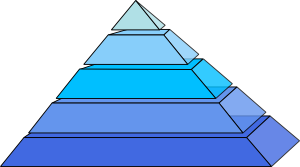
\includegraphics[width=1.1cm]{../Strukturfiler/FIGS/BluePyramid} & \begin{minipage}{\obsl}}{\end{minipage}\\ \end{tabular}\vspace{4mm}\newline}


% = Forudsætning = basis
\newenvironment{basis}{\begin{flushleft} \begin{itshape} }{\end{itshape} \end{flushleft}}


% = Opsummering =
\newenvironment{summary}{\clearpage\pagecolor{sumgul}\section{Opsummering}}{\newpage\pagecolor{white}}











% = Counter
\newcounter{opgavecount}[section]
\setcounter{opgavecount}{0}
\newcounter{spgcount}[opgavecount]
\setcounter{spgcount}{0}
\renewcommand{\thespgcount}{\alph{spgcount})}



% = EXERCISE = (DIVIDER)

\newcommand{\exercisebegin}[1][]{\bigskip\needspace{3\baselineskip}\refstepcounter{opgavecount}\titlegraphic{mingroen}\textcolor{mingroen}{\th{Opgave \theopgavecount \hspace*{1cm} #1}}\medskip\par}

% = QUIZEXERCISE = (DIVIDER)

\newcommand{\quizexercisebegin}[1][]{\bigskip\needspace{3\baselineskip}\refstepcounter{opgavecount}\titlegraphic{mingroen}\textcolor{mingroen}{\th{Quiz-Opgave \theopgavecount \hspace*{1cm} #1}}\medskip\par}

% = QUESTION =

\newenvironment{question}{\refstepcounter{spgcount}\begin{itemize}\item[\thespgcount]}{\end{itemize}\hspace*{\fill}}

% = VINK =

\newenvironment{vink}{\begin{tabular}{m{.9cm}<{\hspace*{2mm}}@{}|m{\obsl}@{}}\hspace*{-4pt}\raggedleft
\includegraphics[width=.9cm]{../Strukturfiler/FIGS/Think} & \begin{minipage}{\obsl}}{\end{minipage}\\ \end{tabular}\medskip\\}
	
% = FACIT =

\newenvironment{facit}{\begin{tabular}{m{.9cm}<{\hspace*{2mm}}@{}|m{\obsl}@{}}\hspace*{-4pt}\raggedleft
\includegraphics[width=.9cm]{../Strukturfiler/FIGS/Check} & \begin{minipage}{\obsl}}{\end{minipage}\\ \end{tabular}\medskip\\}








\newcommand{\afsnit}[1]{\bigskip\th{\titlegraphic{mingroen}\textcolor{mingroen}{#1}} \\ \rule[7pt]{.4\textwidth}{1pt} \vspace*{-2.5mm}\par}

% (DIVIDER):
\newcommand{\ugedagdatotitel}[4]{\pagebreak[4]\section{Semesteruge #1 -- #2 Dag \hspace*{1mm} (#3)} \vspace*{-4mm} \rule[5pt]{\textwidth}{1pt}\vspace*{-2.5mm} \begin{center}\large{\th{#4}}\end{center} \fancyhead[C]{\th{Semesteruge #1}}}

\newenvironment{skema}[1]{\definecolor{shadecolor}{rgb}{0.96,.98, 1.0} \setlength{\FrameSep}{6pt} \renewcommand{\FrameHeightAdjust}{10pt} \vspace*{-4pt}\begin{shaded} \begin{tabular}{#1}}{\end{tabular} \end{shaded} \vspace*{-7pt}}


% ========================

% MAKROER

%\newenvironment{matr}[1][]{\hspace*{-.8mm}\left[\hspace*{-1mm}\begin{array}{#1}}{\end{array}\hspace*{-1mm}\right]\hspace*{-.8mm}}
\newcommand{\bevisslut}{\begin{scriptsize} \begin{flushright} $ \blacksquare $ \end{flushright} \end{scriptsize}}

\newcommand{\tref}[2]{\hyperref[#1]{#2 \ref*{#1}}}
\newcommand{\thref}[2]{\hyperref[#1]{#2}}

\newcommand{\refA}[1]{\colorbox{yellow}{\ref{#1}}}
\newcommand{\hrefA}[2]{\colorbox{yellow}{\href{#1}{#2}}}
\newcommand{\trefA}[2]{\colorbox{yellow}{\hyperref[#1]{#2 \ref*{#1}}}}
\newcommand{\threfA}[2]{\colorbox{yellow}{\hyperref[#1]{#2}}}

\newenvironment{matr}[1]{\hspace*{-.8mm}\begin{bmatrix}\hspace*{-1mm}\begin{array}{#1}}{\end{array}\hspace*{-1mm}\end{bmatrix}\hspace*{-.8mm}}
\newcommand{\transp}{\hspace*{-.6mm}^{\top}}

\newcommand{\maengde}[2]{\left\lbrace \hspace*{-1mm} \begin{array}{c|c} #1 & #2 \end{array} \hspace*{-1mm} \right\rbrace}

\newenvironment{eqnalign}[1]{\setlength{\arraycolsep}{1.3pt}\begin{equation}\begin{array}{#1}}{\end{array}\end{equation}\par}
\newcommand{\eqnl}{\setlength{\arraycolsep}{1.3pt}}

\newcommand{\matind}[3]{{_\mathrm{#1}\mathbf{#2}_\mathrm{#3}}}
\newcommand{\vekind}[2]{{_\mathrm{#1}\mathbf{#2}}}
\newcommand{\jac}[2]{{\mathrm{Jacobi}_\mathbf{#1} (#2)}}
\newcommand{\diver}[2]{{\mathrm{div}\mathbf{#1} (#2)}}
\newcommand{\rot}[1]{{\mathbf{rot}\mathbf{(#1)}}}

\newcommand{\am}{\mathrm{am}}
\newcommand{\gm}{\mathrm{gm}}
\newcommand{\E}{\mathrm{E}}
\newcommand{\Span}{\mathrm{span}}
\newcommand{\mU}{\mathbf{U}}

\newcommand{\ms}{\medskip\\}
\newcommand{\bs}{\bigskip\\}

\newcommand{\mA}{\mathbf{A}}
\newcommand{\mB}{\mathbf{B}}
\newcommand{\mC}{\mathbf{C}}
\newcommand{\mD}{\mathbf{D}}
\newcommand{\mE}{\mathbf{E}}
\newcommand{\mF}{\mathbf{F}}
\newcommand{\mK}{\mathbf{K}}
\newcommand{\mI}{\mathbf{I}}
\newcommand{\mM}{\mathbf{M}}
\newcommand{\mN}{\mathbf{N}}
\newcommand{\mQ}{\mathbf{Q}}
\newcommand{\mT}{\mathbf{T}}
\newcommand{\mV}{\mathbf{V}}
\newcommand{\mW}{\mathbf{W}}
\newcommand{\mX}{\mathbf{X}}
\newcommand{\ma}{\mathbf{a}}
\newcommand{\mb}{\mathbf{b}}
\newcommand{\mc}{\mathbf{c}}
\newcommand{\md}{\mathbf{d}}
\newcommand{\me}{\mathbf{e}}
\newcommand{\mn}{\mathbf{n}}
\newcommand{\mr}{\mathbf{r}}
\newcommand{\mv}{\mathbf{v}}
\newcommand{\mw}{\mathbf{w}}
\newcommand{\mx}{\mathbf{x}}
\newcommand{\mxb}{\mathbf{x_{bet}}}
\newcommand{\my}{\mathbf{y}}
\newcommand{\mz}{\mathbf{z}}
\newcommand{\reel}{\mathbb{R}}
\newcommand{\mL}{\bm{\Lambda}} %Lambda-matrix
\newcommand{\mnul}{\bm{0}}
\newcommand{\trap}[1]{\mathrm{trap}(#1)}
\newcommand{\Det}{\operatorname{Det}}
\newcommand{\adj}{\operatorname{adj}}
\newcommand{\Ar}{\operatorname{Areal}}
\newcommand{\Vol}{\operatorname{Vol}}
\newcommand{\Rum}{\operatorname{Rum}}
\newcommand{\diag}{\operatorname{\bf{diag}}}
\newcommand{\bidiag}{\operatorname{\bf{bidiag}}}
\newcommand{\spanVec}[1]{\mathrm{span}\{#1\}}
\newcommand{\Div}{\operatorname{Div}}
\newcommand{\Rot}{\operatorname{\mathbf{Rot}}}

\newcommand{\Jac}{\operatorname{Jacobi}}
\newcommand{\Tan}{\operatorname{Tan}}
\newcommand{\Ort}{\operatorname{Ort}}
\newcommand{\Flux}{\operatorname{Flux}}
\newcommand{\Cmass}{\operatorname{Cm}}
\newcommand{\Imom}{\operatorname{Im}}
\newcommand{\Pmom}{\operatorname{Pm}}
\newcommand{\IS}{\operatorname{I}}
\newcommand{\IIS}{\operatorname{II}}
\newcommand{\IIIS}{\operatorname{III}}
\newcommand{\Le}{\operatorname{L}}
\newcommand{\app}{\operatorname{app}}
\newcommand{\M}{\operatorname{M}}
\newcommand{\re}{\mathrm{Re}}
\newcommand{\im}{\mathrm{Im}}

\newcommand{\compl}{\mathbb{C}} %de komplekse tal
\newcommand{\e}{\mathrm{e}} %eksponentialfunktionen. lodret 'e', og altså ikke kursiv ligesom andre bogstaver.





% Medialink: SCREEN: (QRcode) + thumbnail image + link på kodenummer (til qr.dtu.dk)
\newcommand{\onlinemedia}[3]{
	\begin{wrapfigure}{r}{3.2cm} 
		\vspace{-30pt} 
		\vspace{#1pt} 
		\begin{flushright} 
			\includegraphics[width=3cm]{qr/#2.png} 
			\tiny 
			\href{http://qr.dtu.dk/#2}{#2: #3}
			\normalsize  
		\end{flushright} 
		\vspace{-10pt} 
	\end{wrapfigure}
}
\newcommand{\onlinemediathumb}[3]{
	\begin{wrapfigure}{r}{3.2cm} 
		\vspace{-30pt} 
		\vspace{#1pt} 
		\begin{flushright} 
			\includegraphics[width=3cm]{qr/#2.png} 
			\includegraphics[width=3cm]{qr/#2_thumb.png} 
			\tiny 
			\href{http://qr.dtu.dk/#2}{#2: #3}
			\normalsize  
		\end{flushright} 
		\vspace{-10pt} 
	\end{wrapfigure}
}



% Index:
\usepackage{makeidx}
\makeindex
\newcommand\ind[2]{\index{#1}\textbf{\textit{\textcolor{black}{#2}}}}

% ###SERVER_EXCLUDE_BEGIN###
\externaldocument[NUID17-]{../../enoten/TN01-Talrum/Talrum}
\externaldocument[NUID1-]{../../enoten/TN02-Ligningssystemer/TNdriver}
\externaldocument[NUID2-]{../../enoten/TN03-Matricer_og_Matrixalgebra/Matricer_og_matrixalgebra}
\externaldocument[NUID3-]{../../enoten/TN04-Kvadratiske_matricer/TNdriver}
\externaldocument[NUID11-]{../../enoten/TN05-Determinanter/Determinanter}
\externaldocument[NUID12-]{../../enoten/TN06-GeometriskeVektorer/GeometriskeVektorer}
\externaldocument[NUID18-]{../../enoten/TN07-Vektorrum/VektorRum}
\externaldocument[NUID21-]{../../enoten/TN08-LinAfbildninger/LinAfbildninger}
\externaldocument[NUID23-]{../../enoten/TN09-Egenvaerdier_og_egenvektorer/TNdriver}
\externaldocument[NUID24-]{../../enoten/TN10-Diagonalisering_med_egenvektorer/TNdriver}
\externaldocument[NUID10-]{../../enoten/TN11-1.ordens_differentialligninger/TNdriver}
\externaldocument[NUID13-]{../../enoten/TN12-1.ordens_differentialligningssystemer/TNdriver}
\externaldocument[NUID14-]{../../enoten/TN13-2.ordens_differentialligninger/TNdriver}
\externaldocument[NUID27-]{../../enoten/TN14-Elemenataere_funktioner/Elementaere_Funktioner}
\externaldocument[NUID28-]{../../enoten/TN15-Funktioner2Variable/Funktioner_To_Variable}
\externaldocument[NUID29-]{../../enoten/TN16-Gradienter_og_Tangentplaner/Gradienter_og_Tangentplaner}
\externaldocument[NUID32-]{../../enoten/TN17-Taylor_formler/Taylor_Formler}
\externaldocument[NUID33-]{../../enoten/TN18-Taylor_2Var/Taylor_2Var}
\externaldocument[NUID34-]{../../enoten/TN19-SymMat/SymmetriskeMatricer}
\externaldocument[NUID35-]{../../enoten/TN20-KegleSnit/Keglesnit}
\externaldocument[NUID36-]{../../enoten/TN21-Riemann_Integral/Riemann_01}
\externaldocument[NUID37-]{../../enoten/TN22-Plan_Int/Plan_Int_01}
\externaldocument[NUID39-]{../../enoten/TN23-Flade_Int/Flade_Rum_Int_01}
\externaldocument[NUID40-]{../../enoten/TN24-Vektorfelter/Vektorfelter_01}
\externaldocument[NUID41-]{../../enoten/TN25-Flux/Flux_02}
\externaldocument[NUID42-]{../../enoten/TN26-Gauss/Gauss_01}
\externaldocument[NUID128-]{../../enoten/TN27-Stokes/Stokes_01}
\externaldocument[NUID43-]{../../enoten/TN29-KomplekseTal/KomplekseTal}

\externaldocument[NUID6-]{../../E-math-opgaver/Opgaver/opgU123}
\externaldocument[NUID19-]{../../E-math-opgaver/Opgaver/opgU45}
\externaldocument[NUID20-]{../../E-math-opgaver/Opgaver/opgU678}
\externaldocument[NUID25-]{../../E-math-opgaver/Opgaver/opgU910SD}
\externaldocument[NUID31-]{../../E-math-opgaver/OpgaverF11-U123/opgF123}
% \externaldocument[NUID9-]{../../E-math-opgaver/Opgaver/Dagsordner E10}
% ###SERVER_EXCLUDE_END###


% Begin document and set alternative chapter title:
\begin{document}
\renewcommand{\chaptername}{eNote}

\setcounter{chapter}{9} %SÆT DETTE TAL TIL 1 MINDRE END DET AKTUELLE TRANSFERNOTE-NUMMER!!

%%%%%%%%%%%%%%%%%%%%%%%%%%%%%%%%%%%%%%%%%%%%
%%%%%%%%%%%%%%%%%%%%%%%%%%%%%%%%%%%%%%%%%%%%%
%%% HERFRA SKAL DU SKRIVE ELLER INDSÆTTE %%%%
%%% DEN FIL DU ØNSKER %%%%%%%%%%%%%%%%%%%%%%%
%%%%%%%%%%%%%%%%%%%%%%%%%%%%%%%%%%%%%%%%%%%%%
%%%%%%%%%%%%%%%%%%%%%%%%%%%%%%%%%%%%%%%%%%%%%

\chapter{Similaritet og diagonalisering} \label{tn10}

\begin{basis}
I denne note forklares, hvordan nogle kvadratiske matricer kan diagonaliseres ved hjælp af egenvektorer. Det forudsættes derfor at man ved, hvordan egenværdier og egenvektorer til en kvadratisk matrix bestemmes og desuden er bekendt med tilhørende begreber, så som algebraisk og geometrisk multiplicitet. 
\end{basis}

Hvis vi betragter en lineær afbildning $\,f:V\rightarrow V\,$ af et $n$-dimensionalt vektorrum $V$ ind i sig selv, så vil afbildningsmatricen for $f$ med hensyn til en vilkårlig basis for $f$ være en kvadratisk, $n \times n$ matrix. Er der givet to baser $a$ og $b$ for $V$, er 
%fremgår det af metode XREF at relationen mellem de to tilsvarende $n \times n$
relationen mellem de tilsvarende afbildningsmatricer $\matind aFa$ henholdsvis $\matind bFb$ givet ved
\begin{equation}\label{afbMskifte}
\matind bFb = (\matind aMb)^{-1} \cdot \matind aFa \cdot \matind aMb 
\end{equation}
hvor
$\,\matind aMb = \begin{matr}{cccc} \vekind ab_1 & \vekind ab_2 & \cdots & \vekind ab_n \end{matr}\,$
er basisskiftematricen der skifter fra $b$ til $a$ koordinater.\bs
Af særlig interesse er det, hvis der findes en basis $v$ bestående af egenvektorer for $f\,.$ Lad nemlig $a$ være en vilkårlig basis for $V\,$ og $\matind aFa$ den hertil hørende afbildningsmatrix for $f\,$. Lad endvidere $v$ være en egenvektorbasis for $V$ med hensyn til $f\,.$ Af \tref{NUID23-MainTh}{sætning} i eNote 9 fremgår det at afbildningsmatricen for $f$ med hensyn til $v$-basis er en diagonalmatrix $\mL$ hvori diagonalelementerne er egenværdierne for $f\,.$ Hvis 
$\mV$ betegner basisskiftematricen, som skifter fra $v$-koordinater til $a$-koordinatvektorerne, vil $\mL$ ifølge (\ref{afbMskifte}) fremkomme således
\begin{equation}\label{afbMskifteDiag}
\mL = \mV^{-1} \cdot \matind aFa \cdot \mV\,. 
\end{equation}%\bs
Formel \ref{afbMskifte} og formel \ref{afbMskifteDiag} inspirer naturligt til spørgsmål der tager udgangspunkt i kvadratiske matricer: Hvilke betingelser skal være opfyldt for at to givne kvadratiske matricer kan fortolkes som  afbildningsmatricer for den samme lineære afbildning med hensyn til to forskellige baser? Og hvilke betingelser skal en kvadratisk matrix opfylde for at den er afbildningsmatrix for en lineær afbildning, som i en anden basis har en diagonalmatrix som afbildningsmatrix? Vi studerer først disse spørgsmål i en ren matrixalgebra-opsætning, og vender i sidste delafsnit tilbage til afbildningssynsvinklen. Til dette formål indføres nu begrebet similære matricer.\bs

\section{Similære matricer}

\begin{definition}[Similære matricer]\label{DefSim}
Givet $n\times n$-matricerne $\mA$ og $\mB\,.$ Man siger at $\mA$ er \textit{similær med} $\mB$ hvis der findes en regulær matrix $\mM$ således at
\begin{equation}\label{tn8.defSimilar} 
\mB=\mM^{-1}\,\mA\,\mM\,.
\end{equation}
\end{definition}

\begin{example}[Similære matricer]
Givet matricerne $\,\mA=\begin{matr}{rr}2&3\\3&-4\end{matr}\,$ og $\,\mB=\begin{matr}{rr}8&21\\-3&-10\end{matr}\,.$\bs
Matricen $\,\mM=\begin{matr}{rr}2&3\\1&2\end{matr}\,$ er regulær og har den inverse matrix $\,\mM^{-1}=\begin{matr}{rr}2&-3\\-1&2\end{matr}\,.$\bs Betragt følgende udregning:
$$\begin{matr}{rr}2&-3\\-1&2\end{matr}
\begin{matr}{rr}2&3\\3&-4\end{matr}
\begin{matr}{rr}2&3\\1&2\end{matr}
=\begin{matr}{rr}8&21\\-3&-10\end{matr}\,.$$\bs
Den viser at $\,\mA\,$ er similær med $\,\mB\,$. 
\end{example}

\begin{aha}
Hvis $\mA$ at være similær med $\mB$, så er $\mB$ også  similær med $\mA,$. Hvis vi nemlig sætter $\mathbf N=\mM^{-1}$, så er $\mathbf N$ regulær, og
$$ \mB=\mM^{-1}\,\mA\,\mM
\,\Leftrightarrow\,
\mM\,\mB\,\mM^{-1}=\mA
\,\Leftrightarrow\,
\mA=\mathbf N^{-1}\,\mB\,\mathbf N\,,$$
Derfor bruger man også talemåden: $\mA$ og $\mB$ er \textit{similære matricer}\,.
\end{aha}

\begin{theorem}[Similaritet er transitivt]\label{tn8.thSimilar}
Lad $\mA\,$, $\mB$ og $\mC$ være $n\times n$-matricer. Hvis $\mA$ er similær med $\mB$, og $\mB$ er similær med $\mC\,$, så er $\mA$ similær med $\mC\,.$
 
\end{theorem}

\begin{exercise}
Bevis sætning \ref{tn8.thSimilar}.
\end{exercise}

Om egenværdierne for similære matricer gælder følgende sætning.

\begin{theorem}[Similaritet og egenværdier] \label{saet.sim}
Hvis $ \mA $ er similær med $\mB\,$, har de to matricer identiske egenværdier med de samme tilhørende algebraiske og geometriske multipliciteter.
\end{theorem}
\begin{bevis}
At $ \mA $ og $\mB$ har de samme egenværdier med de samme tilhørende  algebraiske multipliciteter de har det samme karakteristiske polynomium: Lad $\mM$ være en regulær matrix der opfylder $\,\mB = \mM^{-1} \mA \mM\,$, og lad som sædvanlig $\mE$ betegne enhedsmatricen af samme kvadratiske form som de tre nævnte matricer. Så gælder:
\begin{equation}
\begin{aligned}
\det(\mB - \lambda\mE) &= \det(\mM^{-1} \mA \mM - \lambda \mM^{-1} \mE \mM) \\
&= \det(\mM^{-1}(\mA - \lambda\mE)\mM) \\
&= \det(\mA - \lambda\mE)\,.
\end{aligned}
\end{equation}
Hermed vist at de to matricer har samme karakteristiske polynomium og dermed de samme egenværdier med de samme tilhørende  algebraiske multipliciteter. At de har samme egenværdier fremgår i øvrigt af sætning \ref{tn8.thSimilar2}, som vi viser nedenfor: Når $\mA$ og $\mB$ kan repræsentere den samme lineære afbildning $f$ med hensyn til to forskellige baser, har de identiske egenværdier, nemlig egenværdierne for $f$.\bs Men egenværdierne har også de samme geometriske multipliciteter. Dette følger af at egenrummene for $\mA$ og $\mB$ med hensyn til enhver af egenværdierne kan fortolkes som to forskellige koordinatfremstilllinger for dette samme egenrum, nemlig egenrummet for $f$ med hensyn til den pågældende egenværdi 
\end{bevis}
%Lad $\lambda$ være en egenværdi for $\mB\,.$ Så findes egenrummet for $\lambda$ som den fuldstændige løsning til det lineære ligningssystem der har totalmatricen
%\begin{equation}
%\mT=\left[\mB-\lambda \mE\,|\,\mnul \right]\,. 
%\end{equation}
%På grund af similariteten har vi
%\begin{equation}
%\mB\mv=\mM^{-1}\mA\mM\mv
%=\lambda\mv \Leftrightarrow \mA(\mM\mv)=\mM\lambda\mv=\lambda(\mM\mv)\,.
%\end{equation}
%Her har vi opskrevet egenværdi

%.\bs Tilbage står at vise at egenværdierne også har de samme algebraiske multipliciteter. At dette er tilfældet følger af at de har det samme karakteristiske polynomium: Lad $\mM$ være en regulær matrix der opfylder $\,\mB = \mM^{-1} \mA \mM\,$, og lad som sædvanlig $\mE$ betegne enhedsmatricen af samme kvadratiske form som de tre nævnte matricer. Så gælder:
%\begin{equation}
%\begin{aligned}
%\det(\mB - \lambda\mE) &= \det(\mM^{-1} \mA \mM - \lambda \mM^{-1} \mE \mM) \\
%&= \det(\mM^{-1}(\mA - \lambda\mE)\mM) \\
%&= \det(\mA - \lambda\mE) = 0\,.
%\end{aligned}
%\end{equation}
%Det er hermed bevist.
%\end{bevis}

\begin{obs}
Læg mærke til at sætning \ref{saet.sim} siger at to similære matricer har samme egenværdier, men ikke omvendt: at to matricer, som har samme egenværdier, er similære. Der er en forskel, og kun det første udsagn er sandt.
\end{obs}

\begin{obs}
To similære matricer $ \mA $ og $ \mB $ har samme egenværdier, men en egenvektor for den ene er i almindelighed ikke egenvektor for den anden. Men der gælder at hvis $ \mv $ er en egenvektor for $\mA$ tilhørende egenværdien $ \lambda $, så er $\mM^{-1}\mv$ en egenvektor for $\mB$ tilhørende egenværdien $ \lambda $, hvor $\mM$ er den regulære matrix der opfylder $\,\mB = \mM^{-1} \mA \mM\,$. Der gælder nemlig:
\begin{equation}
\mA\mv = \lambda\mv \quad  \Leftrightarrow \quad \mM^{-1} \mA \mv = \mM^{-1} \lambda \mv \quad \Leftrightarrow \quad \mB (\mM^{-1} \mv) = \lambda (\mM^{-1} \mv) \,.
\end{equation}
\end{obs}

\begin{exercise}
Gør rede for at to kvadratiske $n\times n$-matricer er similære, hvis de har identiske egenværdier med samme tilhørende geometriske multipliciteter, og at summen af de geometriske multipliciteter er $n\,$. 
\end{exercise}






\section{Diagonalisering af matricer}

%Vi starter med at redegøre for hvordan egenværdiproblemet kan kaste afgørende nyt lys over \ind{similære matricer}{similære matricer}, som blev indført i eNote 8, jf. \tref{NUID21-secSimilar}{afsnit}.
%Vi minder om at similaritet handler om et særligt forhold mellem tre kvadratiske $n\times n$-matricer $\,\mA\,$, $\,\mB\,$ og $\,\mM\,$. $\,\mA\,$ kaldes similær med   $\,\mB\,$ hvis der findes en regulær matrix $\,\mM\,$ således at 
%\begin{equation*}\label{tn10.defSimilar} 
%\mB=\mM^{-1}\,\mA\,\mM\,.
%\end{equation*}
%\end{definition}
Betragt en matrix $\,\mA\,$ og en regulær matrix $\,\mV\,$ som er givet ved
\begin{equation}\label{exSim1} 
\mA=\begin{matr}{rr}1&-2\\1&4\end{matr}\,\,\,\mathrm{og}\,\,\,\mV=\begin{matr}{rr}-1&-2\\1&1\end{matr}\,.\end{equation}
Da der gælder at
\begin{equation*}\label{exSim2} 
\mV^{-1}\,\mA\,\mV=
\begin{matr}{rr}1&2\\-1&-1\end{matr}
\begin{matr}{rr}1&-2\\1&4\end{matr}
\begin{matr}{rr}-1&-2\\1&1\end{matr}=
\begin{matr}{rr}3&0\\0&2\end{matr}\,,\end{equation*}
besidder $\,\mA\,$ en særlig egenskab: den er similær med en diagonalmatrix, nemlig diagonalmatricen
$$
\mL=\begin{matr}{rr}3&0\\0&2\end{matr}\,.$$
Man siger i den forbindelse at $\,\mA\,$ er blevet \ind{diagonalisering}{diagonaliseret ved similartransformation}.\bs
Vi vil nu for en vilkårlig given kvadratisk matrix $\,\mA\,$ stille spørgsmålet om den kan diagonaliseres ved similartransformation eller ej. Vi opstiller derfor ligningen 
\begin{equation*}\label{simLign}
\mV^{-1}\,\mA\,\mV=\mL,
\end{equation*}
hvor $\,\mV\,$ er en regulær matrix og $\,\mL\,$ en diagonalmatrix. Vi beviser nedenfor at ligningen har en løsning netop hvis søjlerne i $\,\mV\,$ er lineært uafhængige egenvektorer for $\,\mA\,$, og diagonalelelementerne i $\,\mL\,$ er egenværdierne for $\,\mA\,$ opført således at den $i$-te søjle i $\,\mV\,$ er egenvektor hørende til egenværdien den $i$-te søjle i $\,\mL\,$.\bs
Vi bemærker at dette er i overensstemmelse med eksempel-matricerne i (\ref{exSim1}) ovenfor:
\begin{equation}\label{simLignA}
\begin{matr}{rr}1&-2\\1&4\end{matr}
\begin{matr}{r}-1\\1\end{matr}=
\begin{matr}{r}-3\\3\end{matr}=
3\begin{matr}{r}-1\\1\end{matr}\end{equation}
og
\begin{equation}\label{simLignB}
{\,\,\,}\begin{matr}{rr}1&-2\\1&4\end{matr}
\begin{matr}{r}-2\\1\end{matr}=
\begin{matr}{r}-4\\2\end{matr}=
2\begin{matr}{r}-2\\1\end{matr}\,.\end{equation}
Vi ser i (\ref{simLignA}) at første søjle i $\,\mV\,$ som forventet er egenvektor for $\,\mA\,$ hørende til det første diagonalelement i $\mL$, og vi ser i (\ref{simLignB}) at den anden søjle i $\,\mV\,$ er egenvektor hørende til det andet diagonalelement i $\mL$.

%Vi samler disse overvejelser i den følgende sætning:

\begin{theorem}[Diagonalisering ved similartransformation] \label{saet.diag}
Hvis en kvadratisk matrix $n\times n$-matrix $\,\mA\,$ har $ n $ lineært uafhængige egenvektorer $\, \mv_1, \mv_2, \ldots, \mv_n \,$ respektivt tilhørende de $n$ (ikke nødvendigvis forskellige) egenværdier $\lambda_1, \lambda_2, \ldots, \lambda_n\,$ kan den diagonaliseres ved similartransformationen 
\begin{equation}
\mV^{-1} \mA \mV = \mL \quad \Leftrightarrow \quad \mA = \mV \mL \mV^{-1} \, ,
\end{equation}
hvor
\begin{equation}
\mV = \begin{matr}{cccc} \mv_1 & \mv_2 & \cdots & \mv_n \end{matr} \quad \mathrm{og} \quad \mL = \diag(\lambda_1, \lambda_2, \ldots, \lambda_n) \, .
\end{equation}
Hvis $\,\mA\,$ ikke har $ n $ lineært uafhængige egenvektorer, kan den ikke diagonaliseres ved similartransformation.
\end{theorem}

\begin{bevis}
Antag at $ \mA$ har $n$ lineært uafhængige egenvektorer 
$ \mv_1, \mv_2, \ldots, \mv_n $, og at $\mv_i$ for $i=1\ldots n$ hører til egenværdien $\lambda_i$. Så gælder de følgende $n$ ligninger:

\begin{equation}
\mA\mv_1 = \lambda_1 \mv_1 \quad , \quad \mA\mv_2 = \lambda_2 \mv_2 \quad , \quad \ldots \quad , \quad \mA\mv_n = \lambda_n \mv_n
\end{equation}
De $ n $ ligninger kan samles i et ligningssystem:
\begin{equation} \label{eq.diag}
\begin{aligned}
\begin{matr}{cccc} \mA\mv_1 & \mA\mv_2 & \cdots & \mA\mv_n \end{matr} &= \begin{matr}{cccc} \mv_1 \lambda_1 & \mv_2 \lambda_2 & \cdots & \mv_n \lambda_n \end{matr} \\
\Leftrightarrow \; \mA \begin{matr}{cccc} \mv_1 & \mv_2 & \cdots & \mv_n \end{matr} &= \begin{matr}{cccc} \mv_1 & \mv_2 & \cdots & \mv_n \end{matr} \begin{matr}{cccc} \lambda_1 & 0 & \cdots & 0 \\ 0 & \lambda_2 & \cdots & 0 \\ \vdots & \vdots & \ddots & \vdots \\ 0 & 0 & \cdots & \lambda_n \end{matr} \\
\Leftrightarrow \; \mA \mV &= \mV \mL
\end{aligned}
\end{equation}
Nu er alle egenvektorerne indsat (lodret efter hinanden) i matricen $ \mV $ i samme rækkefølge som egenværdierne er i diagonalen af matricen $ \mL $, som udenfor diagonalen kun indeholder nuller. Da egenvektorerne er lineært uafhængige er matricen $ \mV $ regulær. Derfor findes den inverse $ \mV^{-1} $, og den ganges på fra venstre på begge sider af lighedstegnet:
\begin{equation}
\mV^{-1} \mA \mV = \mV^{-1} \mV \mL \; \Leftrightarrow \; \mV^{-1} \mA \mV = \mL\,.
\end{equation}
Hermed er første del af af sætningen vist. Antag omvendt at $ \mA $ kan diagonaliseres ved en similartransformation. Så findes der en regulær matrix $ \mV=\begin{matr}{cccc} \mv_1 & \mv_2 & \cdots & \mv_n \end{matr} $ og en diagonalmatrix $ \mL=\mathbf {diag}(\lambda_1,\lambda_2,\ldots \lambda_n) $ således at
\begin{equation} \label{tn10.bagfra}
\mV^{-1} \mA \mV = \mL\,.
\end{equation}
Hvis vi nu gentager omformingerne i første del af beviset  blot i modsat rækkefølge, ses det at (\ref{tn10.bagfra}) er ensbetydende med de følgende $n$ ligninger:
\begin{equation}
\mA\mv_1 = \lambda_1 \mv_1 \quad , \quad \mA\mv_2 = \lambda_2 \mv_2 \quad , \quad \ldots \quad , \quad \mA\mv_n = \lambda_n \mv_n
\end{equation}
hvoraf det fremgår at $\mv_i$ for $i=1\ldots n$ er en egenvektor for $ \mA $ tilhørende egenværdien $ \lambda_i $. \bs
Diagonalisering ved similartransformation kan derfor kun opnås på den måde der er omtalt i sætningens første del.
\end{bevis}

Den følgende sætning kan være til stor hjælp når man i forskellige sammenhænge undersøger om matricer kan diagonaliseres ved similartransformation. Hovedresultatet har vi allerede givet i sætning \ref{saet.diag}, men her  forfines betingelserne idet vi trækker på tidligere viste sætninger om egenværdiproblemet for lineære afbildninger og matricer.

\begin{theorem}[Matricers diagonaliserbarhed]\label{diagonaliserbarhed}
For en given $n\times n$-matrix $ \mA $ gælder:\bs
 $ \mA $ kan diagonaliseres ved similartransformation 
\begin{enumerate}
\item
hvis der findes $n$ forskellige egenværdier for  $ \mA\,$.
\item
 hvis summen af egenværdiernes geometriske multipliciteter er $\,n\,$.
\end{enumerate}
 $ \mA $ kan \textit{ikke} diagonaliseres ved similartransformation 
\begin{enumerate}
\setcounter{enumi}{2}
\item
hvis summen af egenværdiernes geometriske multipliciteter er mindre end $n\,$.
\item
hvis der findes blot én egenværdi $\lambda$ med $\,\mathrm{gm}(\lambda)<\mathrm{am}(\lambda)\,$.
%\item
%hvis summen af egenværdiernes algebraiske multipliciteter er mindre end $n\,$.
\end{enumerate}
\end{theorem}
\begin{bevis}
Ad. 1. Hvis der vælges en egentlig egenvektor fra hvert af de $n$ egenrum, følger det af  \tref{NUID23-th.evLinUafh}{hjælpesætning} at det samlede sæt af $n$ egenvektorer er lineært uafhængigt. Derfor kan $\,\mA\,$ ifølge sætning \ref{saet.diag} diagonaliseres ved similartransformation.\bs
Ad. 2:
Hvis der vælges en basis for hvert af egenrummene, så er det samlede sæt af de valgte $n$ egenvektorer ifølge \tref{NUID23-th.evLinUafh}{hjælpesætning} lineært uafhængigt. Derfor kan $\,\mA\,$ ifølge sætning \ref{saet.diag} diagonaliseres ved similartransformation .\bs
Ad. 3:
Hvis summen af de geometriske multipliciteter er mindre en $n$, findes der ikke $n$ lineært uafhængige egenvektorer for. Derfor kan $\,\mA\,$ ifølge sætning \ref{saet.diag} ikke diagonaliseres ved similartransformation. \bs 
Ad. 4:
Da der i følge \tref{NUID23-saet.reg}{sætning} pkt. 1 gælder at summen af de algebraiske multipliciteter højst er $n$, og da der ifølge samme sætning pkt. 2 for enhver egenværdi $\lambda$ gælder at $\,\mathrm{gm}(\lambda)\leq \mathrm{am}(\lambda)\,$, kan summen af de geometriske multipliciteter ikke blive $n$, hvis blot én af egenværdiernes geometriske multiplicitet er mindre end dens algebraiske. Derfor kan $\,\mA\,$ ifølge  det i netop beviste ikke diagonaliseres ved similartransformation.
%Ad. 5:
%Hvis summen af de algebraiske multipliciteter er mindre end $n\,$, må summen af de geometriske i følge \tref{NUID23-saet.reg}{sætning} pkt. 2 også være mindre end $n\,$. Derfor kan $\,\mA\,$ ifølge sætning \ref{saet.diag} ikke diagonaliseres ved similartransformation. 
\end{bevis}


\begin{info}
Et typisk særtilfælde er at en kvadratisk $n\times n$-matrix har i alt $ n $ forskellige egenværdier. Sætning \ref{diagonaliserbarhed} pkt. 1 sikrer at alle matricer af denne type kan diagonaliseres ved similartransformation.
\end{info}

I de følgende eksempler skal vi se, hvordan man konkret kan undersøge om diagonalisering ved similartransformation er mulig og i givet fald gennemføre den.

\begin{example} \label{eks.firstdiag}
Den kvadratiske matrix
\begin{equation}
\mA = \begin{matr}{rrr} 5 & 3 & 2 \\ 2 & 10 & 4 \\ 2 & 6 & 8 \end{matr}
\end{equation}
har egenværdierne $ \lambda_{1}=4 $ og $ \lambda_2 = 15\,.$ $ \mv_1 = (-2,0,1) $ og $ \mv_2 = (-3,1,0) $ er lineært uafhængige vektorer der hører til $ \lambda_{1}$ og $ \mv_3 = (1,2,2) $ er en egentlig egenvektor der hører til $ \lambda_{2}$. Det samlede sæt af de tre nævnte egenvektorer er lineært uafhængigt ifølge  \tref{NUID23-th.evLinUafh}{hjælpesætning}. Det er derfor ifølge sætning \ref{saet.diag} muligt at diagonalisere $ \mA $, fordi der findes $ n = 3 $ lineært uafhængige egenvektorer. Man kan derfor skrive at $ \mL = \mV^{-1} \mA \mV $, hvor
\begin{equation}
\mL = \begin{matr}{rrr} \lambda_1 & 0 & 0 \\ 0 & \lambda_1 & 0 \\ 0 & 0 & \lambda_2 \end{matr} = \begin{matr}{rrr} 4 & 0 & 0 \\ 0 & 4 & 0 \\ 0 & 0 & 15 \end{matr} \quad \mathrm{og} \quad \mV = \begin{matr}{ccc} \mv_1 & \mv_2 & \mv_3 \end{matr} = \begin{matr}{rrr} -2 & -3 & 1 \\ 0 & 1 & 2 \\ 1 & 0 & 2 \end{matr}\,.
\end{equation}
\end{example}

\section{Kompleks diagonalisering}

Hvad vi indtil nu har sagt om similære matricer gælder generelt for kvadratiske, \textit{komplekse} matricer. Grundligningen for diagonalisering ved similartransformation: 
\begin{equation*}\label{simLignKompl}
\mV^{-1}\,\mA\,\mV=\mL,
\end{equation*}
skal derfor forstås i bredest mulig forstand, hvor matricerne $\,\mA,\,\mV\,$ og $\,\mL\,$ er komplekse $n\times n$-matricer. Indtil nu har vi indskrænket os til reelle eksempler, det vil sige eksempler hvor det har været muligt at opfylde grundligningen (\ref{simLignKompl})med reelle matricer. Vi vil i det følgende beskæftige os med en særlig situation, som er typisk i tekniske anvendelser af diagonalisering: Til en given \textit{reel} $n\times n$ matrix $\mA$ søges en regulær matrix $\mM$ og en diagonalmatrix $\mL$ som opfylder grundligningen i bred ramme hvor $\mM$ og $\mL$ muligvis er komplekse (ikke reelle) $n\times n$ matricer.\bs

Det følgendee eksempel viser en reel $3 \times 3$ matrix som ikke kan diagonaliseres reelt fordi dens karakteristiske polynomium kun har én reel rod. Til gengæld kan den diagonailseres komplekst. 

\begin{example}[Kompleks diagonalisering af reel matrix] \label{eks.firstdiag}
Den kvadratiske matrix
\begin{equation}
\mA = \begin{matr}{rrr} 2 & 0 & 5 \\ 0 & 0 & 1 \\ 0 & -1 & 0 \end{matr}
\end{equation}
har egenværdierne $ \lambda_{1}=2\,$, $ \lambda_2 = -i\,$ og $ \lambda_3 = i\,.$ $ \mv_1 =(1,0,0)$ er en egentlig egenvektor der hører til $ \lambda_{1}\,, $ $\mv_2 = (-2+i,i,1) $ en egentlig egenvektor der hører til $ \lambda_{2}\,, $ og $\mv_3 = (-2-i,-i,1) $ en egentlig egenvektor der hører til $ \lambda_{3}\,$. Det samlede sæt af de tre nævnte egenvektorer er lineært uafhængigt ifølge  \tref{NUID23-th.evLinUafh}{hjælpesætning}. Det er derfor ifølge sætning \ref{saet.diag} muligt at diagonalisere $ \mA $. Man kan derfor skrive $ \mL = \mV^{-1} \mA \mV $, hvor
\begin{equation}
\mL = \begin{matr}{rrr} \lambda_1 & 0 & 0 \\ 0 & \lambda_2 & 0 \\ 0 & 0 & \lambda_3 \end{matr} = \begin{matr}{rrr} 2 & 0 & 0 \\ 0 & -i & 0 \\ 0 & 0 & i \end{matr} \quad \mathrm{og} \quad \mV = \begin{matr}{ccc} \mv_1 & \mv_2 & \mv_3 \end{matr} = \begin{matr}{ccc} 1 & -2+i & -2-i \\ 0 & i & -i \\ 0 & 1 & 1 \end{matr}\,.
\end{equation}
\end{example}

Det næste eksempel viser en reel, kvadratisk matrix som ikke kan diagonaliseres, hverken reelt eller komplekst. 


\begin{example}[Ikke-diagonaliserbar kvadratisk matrix]
Givet den kvadratiske matrix
\begin{equation}
\mA = \begin{matr}{rrr} 4 & 1 & -2 \\ 1 & 4 & 1 \\ 0 & 0 & 3 \end{matr} \, ,
\end{equation}
og $ \mA $ har egenværdierne  $ \lambda_{1}= 3 $ og $ \lambda_3 = 5 $. Egenværdien $3$ har den algebraiske multiplicitet 2, men der kun vælges én lineært uafhængig egenvektor, for eksempel $ \mv_1 = (1,-1,0) $. Egenværdien har altså geometrisk multiplicitet 1. Derfor er det ifølge sætning \ref{saet.diag} ikke muligt at diagonalisere $ \mA $ ved similartransformation.
\end{example}

\begin{exercise}
Til matricen
\begin{equation}
\mA = \begin{matr}{rr} 2 & 9 \\ 1 & -6 \end{matr}
\end{equation}
ønskes følgende bestemt:
\begin{enumerate}
\item Alle egenværdier og deres algebraiske multipliciteter.
\item Samtlige tilhørende lineært uafhængige egenvektorer og derved egenværdiernes geometriske multipliciteter.
\item Hvis det er muligt, skal $ \mA $ diagonaliseres: Bestem en diagonalmatrix $ \mL $ og en regulær matrix $ \mV $, hvorom der gælder, at $ \mV^{-1}\mA \mV = \mL $. Hvilke krav er der for at diagonaliseringen kan lade sig gøre? Hvilke tal og vektorer indgår i $ \mL $ og $ \mV\, $?
\end{enumerate}
\end{exercise}

\section{Diagonalisering af lineære afbildninger}
I indledningen til den eNote stillede vi spørgsmålet: Hvilke betingelser skal være opfyldt for at to givne kvadratiske matricer kan fortolkes som afbildningsmatricer for den samme lineære afbildning med hensyn til to forskellige baser? Svaret er enkelt:

\begin{theorem}[Similære matricer som afbildningsmatricer]\label{tn8.thSimilar2}
Der er givet et $\,n$-dimensionalt vektorrum $V\,$. To $\,n\times n\,$ matricer $\mA$ og $\mB$ er afbildningsmatricer for den samme lineære afbildning $\,f:V\rightarrow V\,$ med hensyn til to forskellige baser for $V$, hvis og kun hvis  $\mA$ og $\mB$ er similære.
\end{theorem}

\begin{exercise}
Bevis sætning \ref{tn8.thSimilar2}
\end{exercise}

I indledningen spurgte vi også: Og hvilke betingelser skal en kvadratisk matrix opfylde for at den er afbildningsmatrix for en lineær afbildning, som i en anden basis har en diagonalmatrix som afbildningsmatrix? Svaret fremgår af sætning \ref{saet.diag} kombineret med sætning \ref{tn8.thSimilar2}: Matricen skal have $n$ lineært uafhængige egenvektorer.\bs

Vi slutter eNoten af med et eksempel på diagonalisering af en lineær afbildning, det vil sige finder en passende basis med hensym til hvilken der afbildningsmatrix er en diagonalmatrix.

\begin{example}[Diagonalisering af lineær afbildning]
En lineær afbildning $ f: P_1(\reel) \rightarrow P_1(\reel) $ er givet med følgende afbildningsmatrix med hensyn til standard monomiebasis m:
\begin{equation}
\matind mFm = \begin{matr}{rr} -17 & -21 \\ 14 & 18 \end{matr}
\end{equation}
Det betyder, at $ f(1) = -17 + 14x $ og $ f(x) = -21 + 18x $. Det ønskes undersøgt, om der findes en (reel) egenbasis for $ f $ og i bekræftende tilfælde, hvordan afbildningsmatricen ser ud med hensyn til denne basis, og hvad basisvektorerne er. \bs
Egenværdierne til $ \matind mFm $ bestemmes:
\begin{equation}
\det\!\left(\begin{matr}{cc} -17-\lambda & -21 \\ 14 & 18-\lambda \end{matr}\right) = \lambda^2-\lambda-12 = (\lambda+3)(\lambda-4) = 0\,.
\end{equation}
Det er allerede nu muligt at bekræfte, at der findes en reel egenbasis til $ f $, da der findes $ 2 = \dim(P_2(\reel)) $ egenværdier, nemlig $ \lambda_1 = -3 $ og $ \lambda_2 = 4 $, som hver har algebraisk multiplicitet 1. Egenvektorer til $ \lambda_1 $ bestemmes:
\begin{equation}
\begin{matr}{cc|c} -17+3 & -21 & 0 \\ 14 & 18+3 & 0 \end{matr} \rightarrow \begin{matr}{rr|c} 1 & \frac{3}{2} & 0 \\ 0 & 0 & 0 \end{matr}
\end{equation}
Det giver en egenvektor $ \vekind mv_1 = (-3,2) $, hvis den frie parameter sættes til 2. Tilsvarende fås den anden egenvektor:
\begin{equation}
\begin{matr}{cc|c} -17-4 & -21 & 0 \\ 14 & 18-4 & 0 \end{matr} \rightarrow \begin{matr}{cc|c} 1 & 1 & 0 \\ 0 & 0 & 0 \end{matr}
\end{equation}
Det giver en egenvektor $ \vekind mv_2 = (-1,1) $, hvis den frie parameter sættes til 1. \bs
Der findes altså en reel egenbasis v til $ f $, der er givet med basisvektorerne $ \vekind mv_1 $ og $ \vekind mv_2 $. Vi har da at
\begin{equation}
\matind mMv = \begin{matr}{rr} -3 & -1 \\ 2 & 1 \end{matr} \quad \mathrm{og} \quad \matind vFv = \begin{matr}{rr} -3 & 0 \\ 0 & 4 \end{matr}
\end{equation}
Basen består af vektorerne $ \mv_1 = -3 + 2x $ og $ \mv_2 = -1 + x $ og afbildningen er meget ``simpel'' med hensyn til denne basis. \bs
Man kan gøre prøve med afbildningen af $ \mv_1 $:
\begin{equation}
\begin{aligned}
f(\mv_1) &= f(-3 + 2x) = -3 \cdot f(1) + 2 \cdot f(x) \\
&= -3 \cdot (-17 + 14x) +2 \cdot (-21 + 18x) \\
&= 9-6x = -3(-3+2x) = -3\mv_1
\end{aligned}
\end{equation}
Det passer!
\end{example}


\end{document} 


